% How the fixed-cloud construction works, in three steps. Drawn before it is
% compared against, because the comparison is unreadable without it.
%
%   compile:  pdflatex fixed_cloud.tex
%
\documentclass[border=10pt]{standalone}
\usepackage{lmodern}
\usepackage{amsmath}
\usepackage{amssymb}
\usepackage{tikz}
\usetikzlibrary{arrows.meta,positioning,calc}
% Shared palette for the population-model figures.
%   ink      body / structure
%   popcol   the patient cloud and anything predicted from it
%   mechcol  the simulator and species-level quantities
%   msrcol   the measurement map (readout-level: gamma, kappa)
%   datacol  reported rows
\definecolor{ink}{HTML}{3A3A3A}
\definecolor{popcol}{HTML}{3B4AA6}
\definecolor{mechcol}{HTML}{2E7D5B}
\definecolor{msrcol}{HTML}{EB811B}
\definecolor{datacol}{HTML}{8C3B4A}


% The same candidate patients in all three panels.
\def\keptpts{(-0.95,0.30),(-0.62,-0.10),(-0.30,0.48),(-0.05,-0.32),(0.22,0.20),%
             (0.50,-0.14),(0.78,0.34),(-0.78,-0.44),(0.05,0.55),(0.42,0.52),%
             (-0.42,0.12),(0.65,-0.42),(-0.18,-0.55),(0.30,-0.50),(0.90,0.02),%
             (-1.08,-0.18)}
\def\droppts{(-1.30,0.60),(1.18,0.52),(-1.22,-0.60),(1.24,-0.38),(0.05,0.84),%
             (-0.55,-0.78),(0.72,0.76),(-0.92,0.70)}

\begin{document}
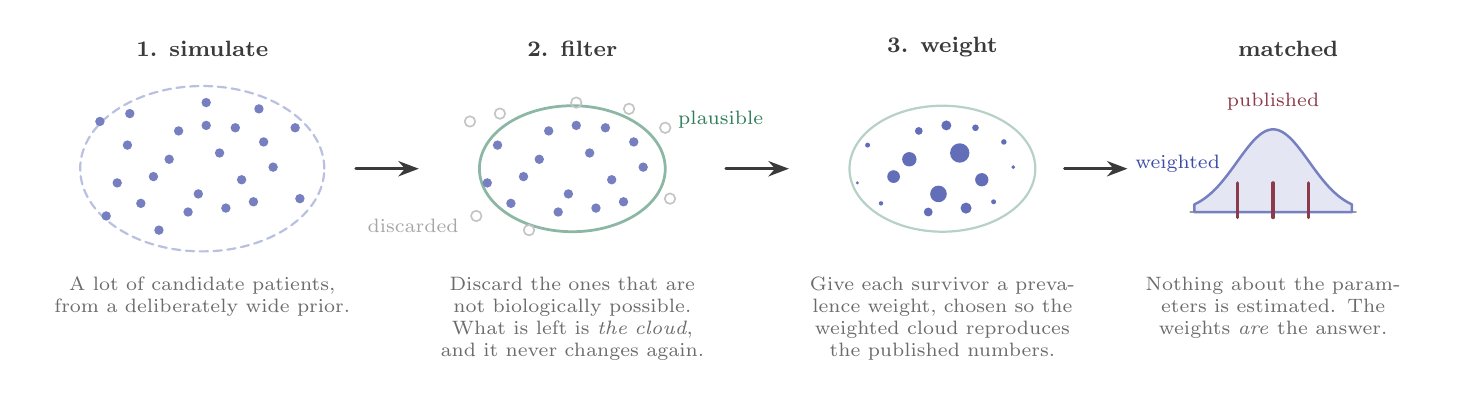
\begin{tikzpicture}[
  font=\sffamily, >=Stealth, line cap=round, line join=round,
  stp/.style={font=\footnotesize\bfseries, text=ink, anchor=south},
  figcap/.style={font=\scriptsize, text=ink!75, align=center, anchor=north,
                 text width=42mm},
  fl/.style={-{Stealth[length=2.6mm]}, ink, line width=1pt}]

% ================================================================ 1. the cloud
\begin{scope}[shift={(0,0)}]
  \draw[popcol!35, densely dashed, line width=0.8pt] (0,0) ellipse (1.55 and 1.05);
  \foreach \p in \keptpts \fill[popcol!70] \p circle (1.7pt);
  \foreach \p in \droppts \fill[popcol!70] \p circle (1.7pt);
  \node[stp] at (0,1.30) {1. simulate};
\end{scope}
\node[figcap] at (0,-1.25)
  {A lot of candidate patients, from a deliberately wide prior.};

\draw[fl] (1.95,0) -- (2.75,0);

% ================================================================ 2. the filter
\begin{scope}[shift={(4.7,0)}]
  \draw[mechcol!55, line width=1pt] (0,0) ellipse (1.18 and 0.80);
  \foreach \p in \keptpts \fill[popcol!70] \p circle (1.7pt);
  \foreach \p in \droppts \draw[ink!30, line width=0.6pt] \p circle (1.9pt);
  \node[mechcol, font=\scriptsize, anchor=west] at (1.22,0.62) {plausible};
  \node[ink!45, font=\scriptsize, anchor=east] at (-1.32,-0.72) {discarded};
  \node[stp] at (0,1.30) {2. filter};
\end{scope}
\node[figcap] at (4.7,-1.25)
  {Discard the ones that are not biologically possible. What is left is
   \emph{the cloud}, and it never changes again.};

\draw[fl] (6.65,0) -- (7.45,0);

% ================================================================ 3. the weights
\begin{scope}[shift={(9.4,0)}]
  \draw[mechcol!35, line width=0.8pt] (0,0) ellipse (1.18 and 0.80);
  \foreach \p/\r in {(-0.95,0.30)/0.9, (-0.62,-0.10)/2.3, (-0.30,0.48)/1.4,
                     (-0.05,-0.32)/3.0, (0.22,0.20)/3.5, (0.50,-0.14)/2.4,
                     (0.78,0.34)/1.0, (-0.78,-0.44)/0.8, (0.05,0.55)/1.8,
                     (0.42,0.52)/1.2, (-0.42,0.12)/2.6, (0.65,-0.42)/0.9,
                     (-0.18,-0.55)/1.6, (0.30,-0.50)/2.0, (0.90,0.02)/0.7,
                     (-1.08,-0.18)/0.6}
    \fill[popcol!80] \p circle (\r pt);
  \node[stp] at (0,1.30) {3. weight};
\end{scope}
\node[figcap] at (9.4,-1.25)
  {Give each survivor a prevalence weight, chosen so the weighted cloud
   reproduces the published numbers.};

\draw[fl] (10.95,0) -- (11.75,0);

% ================================================================ the matching
\begin{scope}[shift={(13.6,0)}]
  \draw[ink!50, line width=0.7pt] (-1.05,-0.55) -- (1.05,-0.55);
  \draw[popcol!70, fill=popcol!14, line width=0.9pt]
    plot[domain=-1.0:1.0,samples=60,smooth] (\x,{-0.55+1.05*exp(-\x*\x/0.42)})
    -- (1.0,-0.55) -- (-1.0,-0.55) -- cycle;
  \foreach \x in {-0.45,0,0.45}
    \draw[datacol, line width=1.2pt] (\x,-0.62) -- (\x,-0.18);
  \node[datacol, font=\scriptsize, anchor=south] at (0,0.62) {published};
  \node[popcol, font=\scriptsize, anchor=north east] at (-0.55,0.30) {weighted};
  \node[stp] at (0,1.30) {\phantom{3.} matched};
\end{scope}
\node[figcap] at (13.6,-1.25)
  {Nothing about the parameters is estimated. The weights \emph{are} the answer.};

\end{tikzpicture}
\end{document}
